% -*- LaTeX -*-
% -*- coding: utf-8 -*-
%
% ~~~~~~~~~~~~~~~~~~~~~~~~~~~~~~~~~~~~~~~~~~~~~~~~~~~~~~~~~~~~~~~~~~~~~~~~~~~~~~
%
%                             michael a.g. aïvázis
%                      california institute of technology
%                      (c) 1998-2010  all rights reserved
%
% ~~~~~~~~~~~~~~~~~~~~~~~~~~~~~~~~~~~~~~~~~~~~~~~~~~~~~~~~~~~~~~~~~~~~~~~~~~~~~~
%

\lecture{Software engineering survival skills}{20100115}

% --------------------------------------
% 
\begin{frame}[fragile]
%
  \frametitle{Software engineering survival skills}
%
  \begin{itemize}
%
  \item class hardware
    \begin{itemize}
    \item your laptop
    \item mind-meld
    \item shc
    \end{itemize}
%
  \item access
    \begin{itemize}
    \item login
    \item shell
    \item setting up the packages you need
    \end{itemize}
%
  \item source control
    \begin{itemize}
    \item why bother?
    \item styles and workflows
    \item available tools
    \end{itemize}
%
  \item writing code
    \begin{itemize}
    \item editing: emacs, vi, ?
    \item compiling and linking
    \item running
    \item testing
    \end{itemize}
%
  \item configuration management
    \begin{itemize}
    \item automating the build process
    \item config
    \end{itemize}
%
  \end{itemize}
%
\end{frame}

% --------------------------------------
% bazaar
\begin{frame}[fragile]
%
  \frametitle{Bazaar -- setup}
%
  \begin{itemize}
%
  \item installation instructions, documentation and tutorials available from
    \href{http://bazaar.canonical.com}
%
  \item bazaar keeps track of authors in its revision history, so it's a good idea to supply
    your name and an email address
%
    \begin{shell}

#> bzr whoami "Michael Aivazis <aivazis@caltech.edu>"
    \end{shell}
%
    \item you should verify that it worked by asking
%
   \begin{shell}

#> bzr whoami
Michael Aivazis <aivazis@caltech.edu>
    \end{shell}
%
  \end{itemize}
%
\end{frame}

% --------------------------------------
% bazaar
\begin{frame}[fragile]
%
  \frametitle{Bazaar -- brances}
%
  \begin{itemize}
%
  \item make a {\em branch} of the course repository by
%
    \begin{shell}

#> bzr branch http://acm114.caltech.edu/repository acm114
Branched 114 revision(s).
    \end{shell}
%
  \item you can look at history with the {\tt\small\bfseries log} command
%
    \begin{shell}

#> bzr log -l10 --line
114: Michael Aivazis 2010-01-14 Started fleshing out 2010.01.15
113: Michael Aivazis 2010-01-14 Posted an updated hw 2010.01.20 with some typos fixed
112: Michael Aivazis 2010-01-13 Created a stub for lecture 2010.01.15
111: Michael Aivazis 2010-01-13 Cosmetics to the reduction parallel work figure
110: Michael Aivazis 2010-01-13 Sidebar cosmetics
109: Michael Aivazis 2010-01-13 Cosmetics on the home page
108: Michael Aivazis 2010-01-13 Cosmetics on the news section of the home page
107: Michael Aivazis 2010-01-13 Published the updated 2010.01.13
106: Michael Aivazis 2010-01-13 Fixed a typo in 2010.01.13
105: Michael Aivazis 2010-01-13 Added news section to the home page
    \end{shell}
%
  \end{itemize}
%
\end{frame}

% --------------------------------------
% repository geometry
\begin{frame}[fragile]
%
  \frametitle{Repository geometry}
%
  \begin{itemize}
%
  \item here's the layout
    \begin{figure}
      \centering
      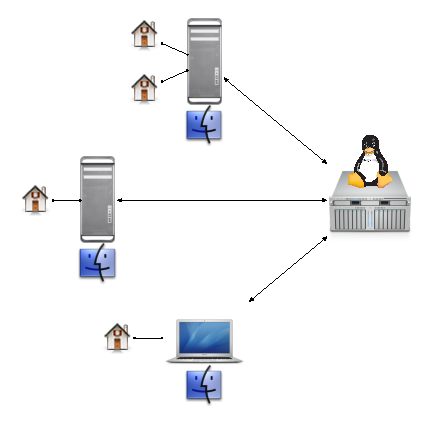
\includegraphics[scale=0.5]{figures/repository-geometry.pdf}
    \end{figure}
%
  \end{itemize}
%
\end{frame}

% end of file 
